\documentclass[10pt]{beamer}
% \documentclass[handout,10pt]{beamer}
\usepackage{my_style}

%%%%%%%%%%%%%%%%%%%%%%%%%%%%%%%%%%%%%%%%%%%%%%%%%%%%%%%%%%%%%%%%%%%%%%%%
%%%%%%%%%%%%%%%%%%%%%%%%%%%%%%%%%%%%%%%%%%%%%%%%%%%%%%%%%%%%%%%%%%%%%%%%

\title[Math/CS 375]{Lecture 13 - A}
\subtitle{\S 8.2, 8.3 Power Method}


\begin{document}
% -------------------------------------------------
\begin{frame}
  \titlepage
\end{frame}

%%%%%%%%%%%%%%%%%%%%%%%%%%%%%%%%%%%%%%%%%%%
\begin{frame}{Goals}
We will answer these questions:\\[3mm]
\begin{itemize}
    \item What are eigenvalues?
    \item What is the power method and what is it used for?
    \item How quickly does power method converge?
    \item How can you modify the power method to find other eigenvalues?
\end{itemize}
\end{frame}
%%%%%%%%%%%%%%%%%%%%%%%%%%%%%%%%%%%%%%%%%%%%%%%%%%%%%%%%%%%%%%%%%%%%%%%%%
\sectionframe{Review Eigenvalues}
\begin{frame}{Eigenvalues, Eigenvectors}
  \begin{itemize}
    \define{Eigenvalues and Eigenvectors}{
    For a matrix $A$, the scalar-vector pairs ($\lambda$, $v$) such that
    \[Av=\lambda v, \qquad v \neq 0\] are \textbf{eigenvalue-eigenvectors}. The pair  ($\lambda$, $v$) is called the \textbf{eigenpair}.      
    }
\item For an $n\times n$ matrix, we expect $n$ eigenvalues 

\item The eigenvalues can be complex even if $A$ contains real numbers 

\item Typically order them $\lambda_1, \lambda_2, \ldots, \lambda_n$ from greatest to least in magnitude\\

\end{itemize}
\end{frame}
%%%%%%%%%%%%%%%%%%%%%%%%%%%%%%%%%%%%%%%%%%%%%%%%%%%%%%%%%%%%%%%%%%%%%%%%%

\begin{frame}{Finding Eigenvalues and Eigenvectors}

\begin{itemize}
   
\begin{example}
Find the eigenvalues and eigenvectors of $ \displaystyle A = \begin{bmatrix} \phantom{-}3 & \phantom{-}2 \\ \phantom{-}7&-2 \end{bmatrix}$
\end{example}

\item First, calculate the \textbf{characteristic equation} $ \det(\lambda I - A)=0$\\
$$
0 = \det(\lambda I-A) = \begin{vmatrix}
    \lambda - 3 & -2\\
    -7 & \lambda+2
\end{vmatrix} = \lambda^2 -\lambda -6 -14 =\lambda^2-\lambda - 20
$$
\item  Find the roots to get the eigenvalues:
$$
0  =\lambda^2-\lambda - 20 = (\lambda-5)(\lambda+4) \implies \lambda_1 = 5 \quad \lambda_2 = -4
$$

  \end{itemize}
\end{frame}
%%%%%%%%%%%%%%%%%%%%%%%%%%%%%%%%%%%%%%%%%%%%%%%%%%%%%%%%%%%%%%%%%%%%%%%%%

\begin{frame}{Finding Eigenvalues and Eigenvectors}

\begin{itemize}
   
\item Solve the system $(\lambda I-A)v_1=0$ with $\lambda_1=5$
$$
5 I - A= 
\begin{bmatrix}
    2 & -2 \\
    -7 & 7
\end{bmatrix} \implies v_1 = \begin{bmatrix}
    1\\1
\end{bmatrix}
$$

\item Solve the system $(\lambda I-A)v_1=0$ with $\lambda_1=-4$
$$
-4 I - A= 
\begin{bmatrix}
    -7 & -2 \\
    -7 & -2
\end{bmatrix} \implies v_2 = \begin{bmatrix}
    -2\\7
\end{bmatrix}
$$
\item \textit{Note}: Any scalar multiple of an eigenvector is an eigenvector

  \end{itemize}
\end{frame}

%%%%%%%%%%%%%%%%%%%%%%%%%%%%%%%%%%%
\begin{frame}{Computing Eigenvalues and Eigenvectors}

\begin{theorem}
    If $v$ is an eigenvector of $A$ then its eigenvalue is 
        $$ \lambda = \frac{(Av)_i}{v_i}$$
\end{theorem}
Proof:
\begin{itemize}
\item By definition we have $Av = \lambda v$ which means
\begin{align*}
    (Av)_i &= (\lambda v)_i \\
    (Av)_i &= \lambda v_i \\
    \implies \lambda &= \frac{(Av)_i}{v_i}
\end{align*}
\end{itemize}
\keyidea{
    If we know a particular eigenvector $v$, then we can find its corresponding eigenvalue $\lambda$ very easily. 
}
\end{frame}

% -----------------

\begin{frame}{Interesting Property}

\begin{theorem}
    If $(v,\lambda)$ is an eigenpair then 
    $$A^nv = \lambda^n v, $$
    where $n$ is any positive integer.
\end{theorem}

    Proof: 
    \begin{itemize}
        \item Start with definition 
        $$A v = \lambda v$$
        \item Multiply both sides by $A$
        $$AAv  = \lambda A v $$
        \item Factor
         $$A(Av) = (Av)\lambda $$
         \item By definition we have 
         $$A^2 v = (\lambda v) \lambda = \lambda^2 v$$
    \end{itemize}
\end{frame}

% --------------------------
\begin{frame}{Eigenvalues?}
\begin{itemize}
    \item Find the eigenvalues of 
    $$A = \begin{bmatrix}
        2 & 0\\ 0 & 2
    \end{bmatrix}$$
    \item Solve $0=\det(\lambda I- A)$
    $$
        0=\det(\lambda I- A) = \begin{vmatrix}
            \lambda - 2& 0 \\ 0 & \lambda-2
        \end{vmatrix} = (\lambda-2)(\lambda-2) \implies \lambda = 2 
     $$

    \item<2> Next, find the eigenvalues of 
    $$B = \begin{bmatrix}
        2 & -1\\ 0 & 2
    \end{bmatrix}$$
    \item<2> Solve $0=\det(\lambda I- B)$
    $$
        0=\det(\lambda I- B) = \begin{vmatrix}
            \lambda - 2& 1 \\ 0 & \lambda-2
        \end{vmatrix} = (\lambda-2)(\lambda-2) \implies \lambda = 2 \text{ same}
     $$
\end{itemize}
\end{frame}

% --------------------------
\begin{frame}{Eigenvectors?}
\begin{itemize}
    \item Find the eigenvectors of 
    $$A = \begin{bmatrix}
        2 & 0\\ 0 & 2
    \end{bmatrix}, \quad \lambda = 2$$
    \item Solve $(\lambda I- A)v=0$
    $$
        \begin{bmatrix}
            \lambda - 2& 0 \\ 0 & \lambda-2
        \end{bmatrix}v = \begin{bmatrix}
            0 & 0 \\
            0 & 0
        \end{bmatrix} v \implies \text{choose } v_1 =\begin{bmatrix}
            1\\0
        \end{bmatrix}, v_2=\begin{bmatrix}
            0\\1
        \end{bmatrix}
     $$
    \item<2> What about 
    $$B = \begin{bmatrix}
        2 & 1\\ 0 & 2
    \end{bmatrix},\quad \lambda=2?$$
    \item<2> Solve $(\lambda I- A)v=0$
    $$
        \begin{bmatrix}
            \lambda - 2& -1 \\ 0 & \lambda-2
        \end{bmatrix}v = \begin{bmatrix}
            0 & -1 \\
            0 & 0
        \end{bmatrix} v \implies \text{only have } v =\begin{bmatrix}
            1\\0
        \end{bmatrix}
     $$
\end{itemize}
\end{frame}

\begin{frame}[fragile]{Diagonalizable}


{
\define{Diagonalizable}{When a matrix $A$ has a full set of independent eigenvectors it is said to be \textbf{diagonalizable}. Otherwise, the matrix is \textbf{deficient}.
}
}

\begin{block}{Matrix $A$ - Diagonalizable}
     $$A = \begin{bmatrix}
        2 & 0\\ 0 & 2
    \end{bmatrix}, \quad \lambda = 2,\quad v_1 =\begin{bmatrix}
            1\\0
        \end{bmatrix},\; v_2=\begin{bmatrix}
            0\\1
        \end{bmatrix}$$
\end{block}
\begin{block}{Matrix $B$ - Deficient}
     $$B = \begin{bmatrix}
        2 & 1\\ 0 & 2
    \end{bmatrix}, \quad \lambda = 2,\quad v =\begin{bmatrix}
            1\\0
        \end{bmatrix}$$
\end{block}

\end{frame}

%%%%%%%%%%%%%%%%%%%%%%%%%%%%%%%%%%%
\sectionframe{Power Method}
%%%%%%%%%%%%%%%%%%%%%%%%%%%%%%%%%%%

\begin{frame}{The Largest Eigenvector}
\begin{itemize}
    \item Suppose that \( A \) is \( n \times n \) and has real eigenvalues
    \[
    |\lambda_1| > |\lambda_2| \geq |\lambda_3| \geq \dots \geq |\lambda_n|
    \]
        \vfill 
    \item Assume $A$ is diagonalizable
        \vfill 
    \item In other words, \( \{v_1, v_2, \ldots, v_n\} \) forms a basis for \( \mathbb{R}^n \).
        \vfill
    
\question{
\begin{itemize}
\item You have $A$. You know it is diagonalizable. 
\item Can you find a way to approximate the dominant eigenvalue $\lambda_1$?
\end{itemize}
}
\end{itemize}
\end{frame}

%%%%%%%%%%%%%%%%%%%%%%%%%%%%%%%%%%%%%%%%%%%

\begin{frame}{Finding the Largest Eigenvalue}{Part 1}
\begin{itemize}
    \item Start with a guess \( x^{(0)} \). Since \( \{v_1, v_2, \ldots, v_n\} \) spans the entire space, we can write
    \[
    x^{(0)} = c_1 v_1 + \dots + c_n v_n
    \]
    \item For simplicity, assume all \( c_j = 1 \):
    \[
    x^{(0)} = v_1 + \dots + v_n
    \]
    \item Now consider the sequence $x^{(i)} = A x^{(i-1)}$:
    \begin{align*}
        x^{(1)} &= A x^{(0)} \\
        x^{(2)} &= A x^{(1)} \\
        x^{(3)} &= A x^{(2)} \\
        &\vdots \\
        x^{(k+1)} &= A x^{(k)}
    \end{align*}
\end{itemize}
\end{frame}

%%%%%%%%%%%%%%%%%%%%%%%%%%%%%%%%%%%%%%%%%%%

\begin{frame}{Finding the Largest Eigenvalue}{Part 2}
\begin{itemize}
    \item With recursion, we can deduce that 
    $$
    x^{(k)} = A^k x^{(0)}
    $$
    \item Using the property $ A^nv = \lambda^n v$, we get
    \begin{align*}
        x^{(k)} &= A^k x^{(0)} \\
                &= A^k ( v_1 + \dots + v_n) \\
                &= \lambda_1^k v_1 + \lambda_2^k v_2 + \dots + \lambda_n^k v_n.
    \end{align*}
    \item Factor out \( \lambda_1^k \):
    \[
    x^{(k)} = \lambda_1^k \left( v_1 + \left(\frac{\lambda_2}{\lambda_1}\right)^k v_2 + \dots + \left(\frac{\lambda_n}{\lambda_1}\right)^k v_n \right)
    \]
\question{
    What happens to $x^{(k)}$ if we let $k\rightarrow \infty$?
}
        
\end{itemize}
\end{frame}

%%%%%%%%%%%%%%%%%%%%%%%%%%%%%%%%%%%%%%%%%%%
\begin{frame}{Finding the Largest Eigenvalue}{Part 3}
\begin{itemize}
    \item Notice that the ratios all have magnitude less than 1
    \[
    x^{(k)} = \lambda_1^k \left( v_1 + \underbrace{\left(\frac{\lambda_2}{\lambda_1}\right)^k}_{\to 0} v_2 + \dots + \left(\frac{\lambda_n}{\lambda_1}\right)^k v_n \right)
    \]
    \item Therefore, in the limit 
    \[ \lim_{k\to\infty} x^{(k)}/\lambda_1^k = v_1 \qquad (c_1=\cdots=c_n=1). \]
    \item The direction of $x^{(k)}$ approaches the line spanned by $v_1$.

\end{itemize}
\end{frame}

%%%%%%%%%%%%%%%%%%%%%%%%%%%%%%%%%%%%%%%%%%%

\begin{frame}[fragile]{The Power Method}

\method{Power Method}
{Given $A$ with independent eigenvectors}
{Largest Eigenvalue $\lambda_1$}
{Extremely simple and efficient method to find $v_1$}

\vspace{6mm}
How it works:
\begin{itemize}
    \item Start with an initial guess whose coefficient of $v_1$ is nonzero. 
    \item Keep multiplying the vector by $A$ 
    \item The direction approaches the line spanned by $v_1$.
\end{itemize}
\vspace{2mm}
If we know an eigenvector, then finding its eigenvalue is nearly free
\end{frame}


%%%%%%%%%%%%%%%%%%%%%%%%%%%%%%%%%%%%%%%%%%%

\begin{frame}[fragile]{The Power Method}

Memory efficient implementation:
\begin{lstlisting}[mathescape]
initialize old
% Use a nonzero component; here we use component 1.
for k=1:kmax
    new = A*old           % get next vector 
    lam = new(1)/old(1)   % estimate eigenvalue 
    old = new             % update 
end
\end{lstlisting}

\vspace{6mm}

\begin{block}{Getting the Eigenvalue}
    Since $x^{(k+1)}  = A x^{(k)}$ and $\lambda = (Av)_i/v_i$, we have the formula 
    $$ \lambda \approx \frac{(A x ^{(k)})_1}{x_1^{(k)}} = \frac{x_1^{(k+1)}}{x_1^{(k)}} $$
\end{block}

\end{frame}

%%%%%%%%%%%%%%%%%%%%%%%%%%%%%%%%%%%%%%%%%%%

\begin{frame}{Power Method by Hand}
\begin{example}
    Approximate the largest eigenvalue of $A = \begin{bmatrix} \phantom{-}3 & \phantom{-}2 \\ \phantom{-}7&-2 \end{bmatrix}$ with two iterations of the power method using the initial guess $x^{(0)} = [1 \quad 0]^T$. 
\end{example}
\begin{itemize}
    \item $x^{(0)} = \begin{bmatrix} 1\\0\end{bmatrix}$
    \item $x^{(1)} = \begin{bmatrix} \phantom{-}3 & \phantom{-}2 \\ \phantom{-}7&-2 \end{bmatrix}\begin{bmatrix} 1\\0 \end{bmatrix} = \begin{bmatrix} 3\\7 \end{bmatrix}$
    \item $x^{(2)} = \begin{bmatrix} \phantom{-}3 & \phantom{-}2 \\ \phantom{-}7&-2 \end{bmatrix}\begin{bmatrix} 3\\7 \end{bmatrix} = \begin{bmatrix} 23\\7 \end{bmatrix}$
    \item $\lambda \approx 23/3 = 7\frac{2}{3}$ (true answer is $\lambda=5$) 
\end{itemize}
    
\end{frame}

%%%%%%%%%%%%%%%%%%%%%%%%%%%%%%%%%%%%%%%%%%%
\sectionframe{Normalization}
%%%%%%%%%%%%%%%%%%%%%%%%%%%%%%%%%%%%%%%%%%%

\begin{frame}{Predict the Next Estimate}
Our first-component estimates were $3$ and $23/3\approx7.67$.
\question{Will the next estimate be above or below $5$?}
\pause
\[
x^{(3)}=\begin{bmatrix}3&2\\7&-2\end{bmatrix}
\begin{bmatrix}23\\7\end{bmatrix}=\begin{bmatrix}83\\147\end{bmatrix},
\qquad \frac{83}{23}\approx3.61.
\]
\keyidea{The estimate crossed $5$ again. What is happening to the direction?}
\end{frame}

\begin{frame}{Watch the Direction}
\begin{columns}[c]
\begin{column}{.50\textwidth}
\centering
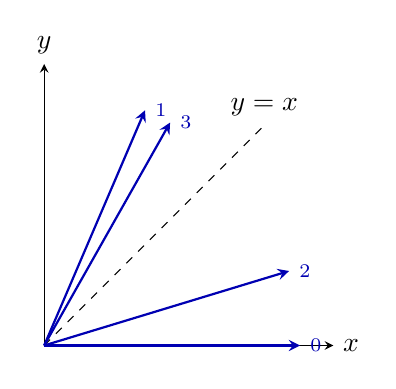
\begin{tikzpicture}[scale=3.25,>=stealth]
\draw[->] (0,0)--(1.13,0) node[right] {$x$};
\draw[->] (0,0)--(0,1.1) node[above] {$y$};
\draw[dashed] (0,0)--(.86,.86) node[above] {$y=x$};
\foreach \u/\v/\k in {1/0/0,.394/.919/1,.957/.291/2,.492/.871/3}
  \draw[blue!70!black,thick,->] (0,0)--(\u,\v) node[right,font=\scriptsize] {$\k$};
\end{tikzpicture}
\end{column}
\begin{column}{.45\textwidth}
Arrows show unit directions; labels give the iteration $k$.

\medskip
The dominant eigenvector lies on $y=x$. Relative to its component, the other eigenvector component is multiplied by
\[
\lambda_2/\lambda_1=-4/5
\]
at each step.
\end{column}
\end{columns}
\keyidea{The sign explains the alternating sides; the magnitude explains why the directions draw closer.}
\end{frame}



%%%%%%%%%%%%%%%%%%%%%%%%%%%%%%%%%%%%%%%%%%%

\begin{frame}[fragile]{Overflow or Underflow}
\begin{itemize}
    \item Eventually, the vector will \textbf{overflow}
\begin{lstlisting}[mathescape]
x =

   Inf
   Inf
\end{lstlisting}

    \item The multiplication causes the magnitude of the vector to grow each time
    $$
    x^{(k)}= A x^{(k-1)}
    $$

    \item On the other hand, if $||A||<1$, then 
    $$
    x^{(k)}= A x^{(k-1)}
    $$
    would cause the vector to shrink and eventually \textbf{underflow}
\end{itemize}
\end{frame}


\begin{frame}{Scale the Vectors}


    \begin{itemize}
        \item We need to iterate to improve
            \vfill 
        \item But iteration leads to overflow/underflow
            \vfill 
        
    
    \begin{block}{The Fix}
    \begin{itemize}
        \item Any constant multiple of an eigenvector is still an eigenvector 
            
        \item We can scale down \( x^{(k)} \) so it doesn't overflow
    \end{itemize}
    \end{block}
    \end{itemize}
    
\end{frame}
%%%%%%%%%%%%%%%%%%%%%%%%%%%%%%%%%%%%%%%%%%%
\begin{frame}{Normalization}

\define{Normalization}{
\textbf{Normalizing} a vector $v$ means scaling it in a way that makes its norm equal to one, e.g.
$$
||cv|| = 1.
$$
}

\begin{itemize}
    \item Example: 
    $$
        v = \begin{bmatrix}
            3\\4
        \end{bmatrix}
    $$
    \item We can use the 2-norm 
    $$
    ||v||_2 = \sqrt{3^2+4^2} = 5
    $$

    \item Scale down by $c=1/5$
    $$
    cv = \frac{1}{5} \begin{bmatrix}
        3\\4
    \end{bmatrix} = \begin{bmatrix}
        3/5\\4/5
    \end{bmatrix}. 
    $$
\end{itemize}
    
\end{frame}

%%%%%%%%%%%%%%%%%%%%%%%%%%%%%%%%%%%%%%%%%%%

\begin{frame}{Norms}

\begin{enumerate}

    \item 2-Norm 
    $$
    \| x \|_2 = \sqrt{x_1^2 + x_2^2 + \dots + x_n^2}
    $$
    \item Infinity norm
    $$ \| x \|_\infty = \max(|x_1|, |x_2|, \dots, |x_n|) $$

    \item 1-Norm 
    $$ \| x \|_1 = |x_1| + |x_2| + \dots + |x_n| $$
    
    \begin{itemize}
        \item Suppose all elements $x_i>0$ 
        \item Then normalizing  
        $$
            \frac{x}{||x||_1}
        $$
        causes the new vector to have elements that add up to 1
    \end{itemize}
    

\end{enumerate}

\end{frame}
%%%%%%%%%%%%%%%%%%%%%%%%%%%%%%%%%%%%%%%%%%%
\begin{frame}{Need for Normalization}
\begin{itemize}
    \item Starting with $x^{(0)}$, if we iterate $x^{(i)} = A x^{(i-1)}$ infinitely... 
    \[ \lim_{k\to\infty} x^{(k)}/\lambda_1^k = v_1 \qquad (c_1=\cdots=c_n=1). \]
    \item If $|\lambda_1| < 1$, then the entire vector converges to zero 
    \item If $|\lambda_1| >1$, then the vector diverges
\end{itemize}

\keyidea{

\begin{itemize}
    \item Simple method $x^{(i)} = A x^{(i-1)}$ will diverge or give us garbage.
    \item But, scaling $x^{(i)} := \frac{A x^{(i-1)}}{\| A x^{(i-1)} \| }$ fixes both issues!
\end{itemize}
}


\end{frame}


\begin{frame}[fragile]{The Power Method (with normalization)}

New algorithm with normalization
\begin{lstlisting}[mathescape]
initialize old
% Use a nonzero component; here we use component 1.
for k=1:kmax
    new = A*old   
    lam = new(1)/old(1)   
    old = new/norm(new,1)    % scale down with 1-norm
end
\end{lstlisting}
\vspace{6mm}
\begin{itemize}
    \item Add one line of code to scale down the vector
    \item Avoid underflow and overflow 
    \item This is the standard power method
\end{itemize}
% \begin{block}{Convergence Rate}
%  Power method converges linearly  
%     $$ E_{k+1} =  \frac{\lambda_2}{\lambda_1}E_{k } \quad \text{or} \quad E_k = \mathcal{O}\left((\lambda_2/\lambda_1)^k\right)$$
% \end{block}
\end{frame}

%%%%%%%%%%%%%%%%%%%%%%%%%%%%%%%%%%%%%%%%%%%%%%%%%%%%%%%%%%%%%%%%%%%%%%%%
\begin{frame}{Convergence Rate}

\begin{theorem}
Let \( A \) have eigenvalues ordered as
\[
|\lambda_1| > |\lambda_2| \ge \cdots \ge |\lambda_n|.
\]
For diagonalizable $A$ and $c_1\ne0$, the error in direction satisfies
\[
E_k = \mathcal{O}\!\left(\left|\frac{\lambda_2}{\lambda_1}\right|^k\right).
\]
\end{theorem}


\vspace{5mm}
\begin{itemize}
    \item The convergence speed depends on the eigenvalue gap
    \item Larger separation between \( |\lambda_1| \) and \( |\lambda_2| \) gives faster convergence
    \item Power method is linearly convergent (not fast, but cheap)
\end{itemize}
\end{frame}
%%%%%%%%%%%%%%%%%%%%%%%%%%%%%%%%%%%%%%%%%%%%%%%%%%%%%%%%%%%%%%%%%%%%%%%%
% \begin{frame}{Convergence Proof Outline}{Part 1}

% \begin{itemize}
%     \item \textbf{Step 1: Express \( x^{(k)} \) in Terms of Eigenvectors.}  
%     Start with an initial vector \( x^{(0)} \) expressed as a combination of eigenvectors:
%     \[
%     x^{(k)} = \lambda_1^k\left( c_1 v_1 + \left(\frac{\lambda_2}{\lambda_1}\right)^k c_2 v_2 + \dots + \left(\frac{\lambda_n}{\lambda_1}\right)^k c_n v_n \right).
%     \]
    
%     \vspace{4mm}
    
%     \item \textbf{Step 2: Define the Error \( E_k \)}.  
%     The error at iteration \( k \) is the difference between \( x^{(k)} \) and the dominant eigenvector \( v_1 \):
%     \[
%     E_k = \left\| v_1 - \frac{x^{(k)}}{\|x^{(k)}\|} \right\|.
%     \]

%     \vspace{4mm}

% \end{itemize}
% \end{frame}
% %%%%%%%%%%%%%%%%%%%%%%%%%%%%%%%%%%%%%%%%%%%%%%%%%%%%%%%%%%%%%%%%%%%%%%%%
% \begin{frame}{Convergence Proof Outline}{Part 2}
% \begin{itemize}
%     \item \textbf{Step 3: Estimate \( E_k \)}.  
%     Using \( x^{(k)} \) expression, we have:
%     \begin{align}
%     E_k &= \left\| v_1 - \lambda_1^k\left( c_1 v_1 + \sum_{i=2}^n \left(\frac{\lambda_i}{\lambda_1}\right)^k c_i v_i \right) \right\| \\     
%         &= \left\| -\sum_{i=2}^n \left(\frac{\lambda_i}{\lambda_1}\right)^k c_i v_i \right\| \\   
%         &\leq \sum_{i=2}^n \left| \frac{\lambda_i}{\lambda_1} \right|^k |c_i| \|v_i\| \\  
%         &\leq M n \left| \frac{\lambda_2}{\lambda_1} \right|^k,
%     \end{align}
%     where \( M \) is a constant dependent on \( \|v_i\| \).
% \end{itemize}
% \end{frame}

%%%%%%%%%%%%%%%%%%%%%%%%%%%%%%%%%%%%%%%%%%%%%%%%%%%%%%%%%%%%%%%%%%%%%%%%
\begin{frame}{Idea Behind the Convergence Rate}

\begin{itemize}
    \item After \( k \) iterations,
    \[
    x^{(k)} = \lambda_1^k\left( c_1 v_1 + \left(\frac{\lambda_2}{\lambda_1}\right)^k c_2 v_2 + \dots + \left(\frac{\lambda_n}{\lambda_1}\right)^k c_n v_n \right).
    \]
    \item If $c_1\ne0$, the scaled error satisfies
    \[
      \left\|x^{(k)}/\lambda_1^k-c_1v_1\right\|
      \le M\left|\frac{\lambda_2}{\lambda_1}\right|^k .
    \] 
    \keyidea{
        The smaller $|\lambda_2/\lambda_1|$ is, the faster the direction converges.
    }
\end{itemize}
\end{frame}

%%%%%%%%%%%%%%%%%%%%%%%%%%%%%%%%%%%%%%%%%%%%%%%%%%%%%%%%%%%%%%%%%%%%%%%%
\begin{frame}{Predict: Which Run Is Faster?}
Start at $x^{(0)}=(1,1)^T$ in both runs.
\[
A=\operatorname{diag}(5,1),\qquad B=\operatorname{diag}(5,4.9).
\]
\question{After ten steps, which vector points closer to the first coordinate axis?}
\pause
For a diagonal matrix, the ratio of the second component to the first is
$(\lambda_2/\lambda_1)^k$, even after normalization.
\[
A:\ (1/5)^{10}\approx10^{-7}
\qquad B:\ (4.9/5)^{10}\approx0.82.
\]
\keyidea{Both runs converge. The ratio of eigenvalue magnitudes decides how fast.}
\end{frame}

\sectionframe{When Does the Power Method Fail?}
\begin{frame}{What If Two Eigenvalues Tie in Magnitude?}
\[
A=\operatorname{diag}(5,-5),\qquad x^{(0)}=(1,1)^T.
\]
\question{Which directions do the next two iterates point in?}
\pause
\[
(1,1)^T \ \longmapsto\ (5,-5)^T \ \longmapsto\ (25,25)^T .
\]
The iterates alternate between $y=-x$ and $y=x$. Normalizing changes their lengths but preserves this cycle.
\keyidea{With a ratio of $-4/5$ the oscillation shrank. With $-5/5=-1$, it persists.}
\end{frame}

\begin{frame}{What If We Start on the Wrong Eigenvector?}
\[
A=\operatorname{diag}(5,1),\qquad x^{(0)}=(0,1)^T.
\]
\question{The vector stops changing immediately. Did we find the dominant eigenpair?}
\pause
\[
A(0,1)^T=(0,1)^T.
\]
We found an exact eigenvector for $\lambda=1$. Its component along the dominant eigenvector $(1,0)^T$ is zero at every step.
\keyidea{For the diagonalizable matrices considered here, check both assumptions: $|\lambda_1|>|\lambda_2|$ and $c_1\ne0$.}
\end{frame}

\begin{frame}{When Should We Stop Iterating?}
For a normalized iterate $x$ and its eigenvalue estimate $\mu$, check the eigenvalue equation:
\[
r=Ax-\mu x.
\]
\begin{itemize}
\item Reuse $y=Ax$ from the iteration. Compute $\mu$ from $y$ and $x$, then test $r=y-\mu x$ before replacing $x$.
\item A small residual means this pair nearly satisfies $Ax=\mu x$. Keep an iteration limit as well.
\end{itemize}
\question{In the preceding example, what is the residual for $\mu=1$?}
\pause
It is zero. A residual checks the eigenpair equation; it cannot certify dominance.
\end{frame}

\sectionframe{Other Eigenvalues}
%%%%%%%%%%%%%%%%%%%%%%%%%%%%%%%%%%%%%%%%%%%%%%%%%%%%%%%%%%%%%%%%%%%%%%%%
\begin{frame}{Smallest Eigenvalue}

{
\question{
    How can we find the eigenvalue of $A$ with smallest magnitude?
}}
    \begin{theorem}
        If $A$ is invertible and $\lambda$ is an eigenvalue of $A$, then $\frac{1}{\lambda}$ is an eigenvalue of $A^{-1}$. 
    \end{theorem}
    Proof: 
    \begin{itemize}
        \item Suppose \( A v = \lambda v \) for some eigenvector \( v \).
        \item Then, multiplying both sides by \( A^{-1} \) gives \( A^{-1} A v = A^{-1} \lambda v \).
        \item Simplifying, we get \( v = \lambda A^{-1} v \) or 
            $$ A^{-1} v = \frac{1}{\lambda} v. $$
        \item By definition, \( \frac{1}{\lambda} \) is an eigenvalue of \( A^{-1} \).
    \end{itemize}
\end{frame}


%%%%%%%%%%%%%%%%%%%%%%%%%%%%%%%%%%%%%%%%%%%%%%%%%%%%%%%%%%%%%%%%%%%%%%%%
\begin{frame}{Reciprocals}

\begin{itemize}
    \item Suppose the eigenvalues of $A$ are
    $$
    \lambda_1 = 10,\quad  \lambda_2 = 5,\quad  \lambda_3 = 2
    $$
    
    \item Then the eigenvalues of $A^{-1}$ must be 

    $$
    \lambda_1 = \frac{1}{2},\quad  \lambda_2 = \frac{1}{5},\quad  \lambda_3 = \frac{1}{10}
    $$
    
    \item<2> Notice that the \textit{smallest} eigenvalue of $A$ is the reciprocal of the \textit{largest} eigenvalue of $A^{-1}$
    $$
    2 \quad \text{ v.s. } \quad \frac{1}{2}
    $$
\end{itemize}

\onslide<2>{
    \keyidea{
       To find the smallest eigenvalue of $A$, do power method on $A^{-1}$
} 
}
\end{frame}

%%%%%%%%%%%%%%%%%%%%%%%%%%%%%%%%%%%%%%%%%%%%%%%%%%%%%%%%%%%%%%%%%%%%%%%%
\begin{frame}{Inverse Power Method}

{
\method{Inverse Power Method}
{Matrix $A$ with independent eigenvectors}
{Smallest eigenvalue in magnitude $\lambda_n$}
{Simply do power method on $A^{-1}$}
}




\vspace{4mm}
Note:
\begin{itemize}
    \item You are \emph{never} supposed to compute $A^{-1}$
    \item Compute a factorization instead
\end{itemize}
\end{frame}

%%%%%%%%%%%%%%%%%%%%%%%%%%%%%%%%%%%%%%%%%%%%%%%%%%%%%%%%%%%%%%%%%%%%%%%%

\begin{frame}[fragile]{Inverse Power Method Algorithm}

\textbf{Algorithm:}
\begin{lstlisting}[mathescape]
factorize A
initialize old
% Use a nonzero component; here we use component 1.
for k=1 to kmax
    new = solve(A, old)       % Solve system A * new = old
    lam = new(1)/old(1)     % Estimate eigenvalue of inverse
    old = new / norm(new,inf)      % Normalize vector
end 

return 1/lam
\end{lstlisting}

\vspace{4mm}

\begin{itemize}
    \item Note: Instead of directly inverting \( A \), we solve \( A \, \texttt{new} = \texttt{old} \) at each iteration, which is more computationally efficient.
    \item This yields the smallest eigenvalue of \( A \), with \( \lambda_{\text{min}} \approx \frac{1}{\texttt{lam}} \).
\end{itemize}
\end{frame}

\begin{frame}{Remarks on the Inverse Power Method}
Why would you want to know $\lambda_n$?
\begin{block}{Condition Number}
    For an invertible real symmetric matrix with eigenvalues ordered by magnitude, the 2-norm condition number is 
        $$\kappa_2(A) = \frac{|\lambda_1|}{|\lambda_n|}.$$
\end{block}
\vspace{3mm}
And the convergence rate?
\begin{block}{Convergence Rate Formula}
    For error \( E_k \) at iteration \( k \), we have:
    \[
    E_k = \mathcal{O} \left( \left| \frac{\lambda_n}{\lambda_{n-1}} \right|^k \right).
    \]
\end{block}
\end{frame}



%%%%%%%%%%%%%%%%%%%%%%%%%%%%%%%%%%%%%%%%%%%%%%%%%%%%%%%%%%%%%%%%%%%%%%%%
\begin{frame}{Other Eigenvalues}
    \begin{itemize}
        \item Power method finds $\lambda_1$
        \item Inverse power method finds $\lambda_n$
        \item There are still $n-2$ other eigenvalues 
        $$ \lambda_2, \lambda_3, \ldots, \lambda_{n-1}$$
        \question{
        
        How do you find the other eigenvalues?
        }
    
        \onslide<2>{
            \item Homework!
        }
    \end{itemize}
\end{frame}

\begin{frame}{Next Week: When Normalization Is Automatic}
Today we rescaled $Ax$ to keep the iterates from growing or shrinking.

\medskip
Next week, $x$ will be a probability vector. Our transition matrix $P$ will preserve nonnegativity and the sum of its entries:
\[
x^{(k+1)}=Px^{(k)},\qquad \sum_i x_i^{(k)}=1.
\]
\question{If this sequence settles to a vector $x$, what equation must $x$ satisfy?}
\pause
\[
Px=x.
\]
\end{frame}
\end{document}
